\documentclass{article}%
\usepackage[T1]{fontenc}%
\usepackage[utf8]{inputenc}%
\usepackage{lmodern}%
\usepackage{textcomp}%
\usepackage{lastpage}%
\usepackage[margin=0.7in]{geometry}%
\usepackage{float}%
\usepackage{ragged2e}%
\usepackage{graphicx}%
\usepackage{fancyhdr}%
%
\fancypagestyle{header}{ 
\renewcommand{\headrulewidth}{0pt}%
\renewcommand{\footrulewidth}{0pt}%
\fancyhead{ 
}%
\fancyfoot{ 
}%
\fancyhead[L]{ 
Center for Reflected Text Analytics (CRETA)\newline%
University of Stuttgart
}%
\fancyhead[R]{ 
\today
}%
\fancyfoot[C]{ 
Page \thepage\ of \pageref{LastPage}
}
}%
%
\begin{document}%
\normalsize%
\pagestyle{header}%
\begin{minipage}{\textwidth}%
\centering%
\begin{Large}%
\textbf{rCAT v0.1}%
\end{Large}%
\linebreak%
\begin{large}%
\textbf{Relational Character Analysis Tool}%
\end{large}%
\end{minipage}%


\begin{figure}[h!]%
\centering%
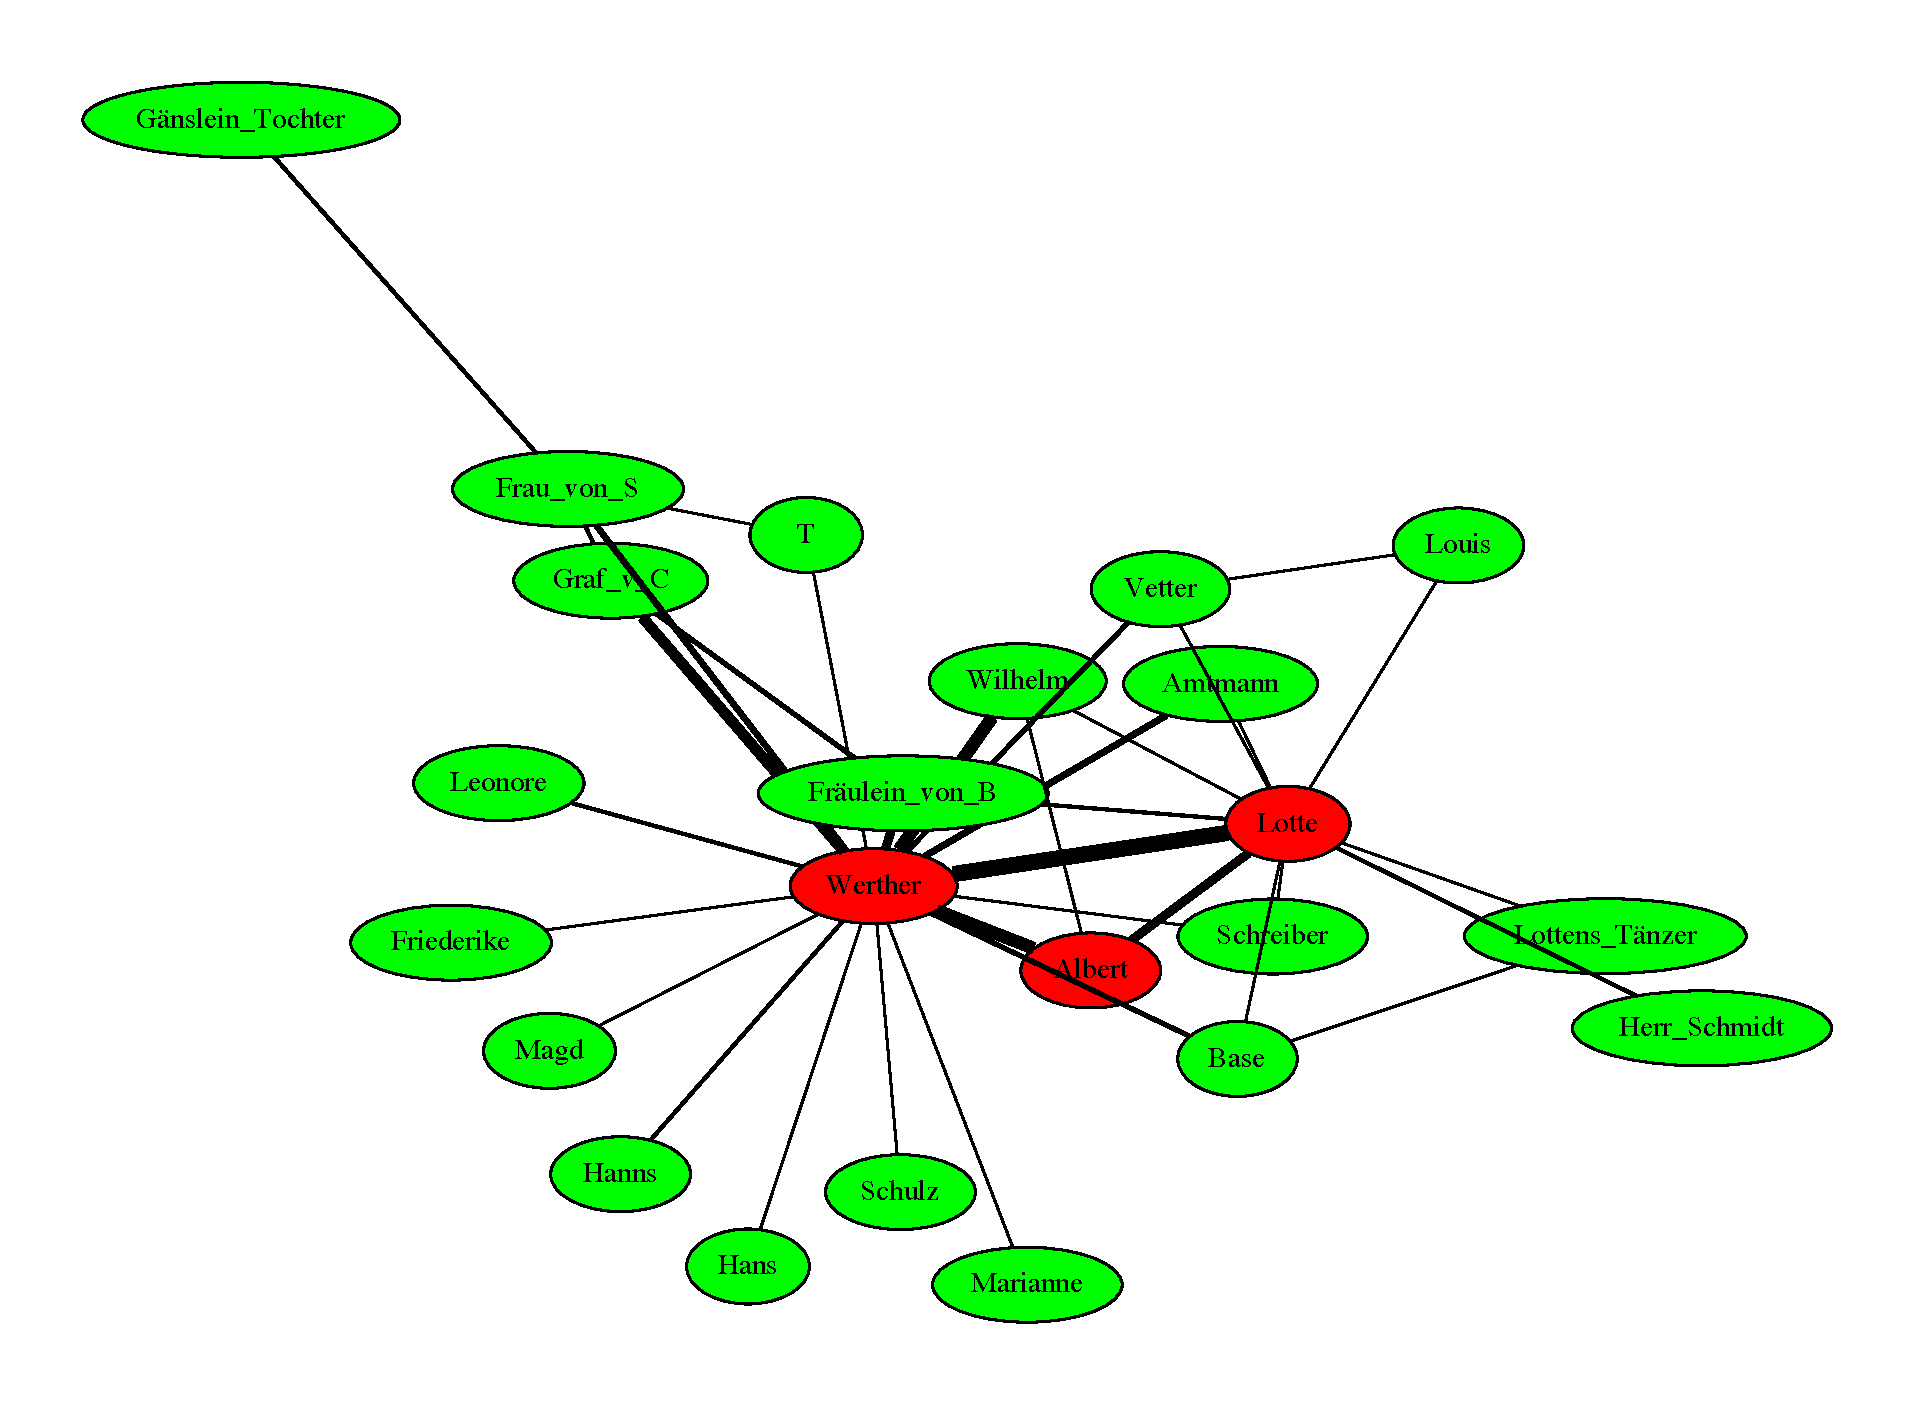
\includegraphics[width=0.8\textwidth]{/Users/Florian 1/Applications/Source_Tree/web-rcat/flask_app/data_user/36bf6974-1bdd-11e8-af65-600308993272_temp_folder/network.pdf}%
\caption{Network}%
\end{figure}

%
\section{Data Input}%
\subsection*{Statistics}%
\begin{itemize}%
\item%
timestamp: 2018{-}02{-}27 17:44:29%
\item%
analyzed text: "1\_\_1\_Mann\_Zauberberg.txt"%
\item%
length of text: 313533 tokens%
\item%
number of characters (with at least one degree): 17%
\end{itemize}

%
\subsection*{Input parameters}%
\begin{itemize}%
\item%
distance measure: 10%
\item%
context measure 1 (words before Character 1): 8%
\item%
context measure 2 (words after Character 2): 8%
\end{itemize}

%
\section{Network Parameters}%
Here you can get information about the network parameters.%
\subsection*{Definitions}%
\begin{itemize}%
\item%
Average degree: The degree of a node is the number of edges connected to it. It measures the number of connections to other characters. Average degree is calculated                        on a probability of two nodes being connected.%
\item%
SD degree: Standard deviation of all degrees.%
\item%
Density: Graph density is the ratio of the number of edges to the number of possible edges.%
\item%
Weighted degree: Sum of weights of incident edges. Measures the number of interactions of a character.%
\end{itemize}

%
\subsection*{Current network parameters}%
\begin{itemize}%
\item%
average degree: 6.235294117647059%
\item%
sd degree: 3.011009211309098%
\item%
density: 0.3897058823529412%
\end{itemize}

%
\subsection*{Degrees}%
\begin{tabular}{|c|c|c|}%
\hline%
Character (Node)&degree&weighted degree\\%
\hline%
Hans Castorp&14&455\\%
\hline%
Settembrini&10&233\\%
\hline%
Naphta&5&125\\%
\hline%
Madame Chauchat&6&80\\%
\hline%
Peeperkorn&5&53\\%
\hline%
Ziemßen&4&33\\%
\hline%
Behrens&5&40\\%
\hline%
Krokowski&4&41\\%
\hline%
Stöhr&10&37\\%
\hline%
Mylendonk&3&7\\%
\hline%
Pribislav Hippe&2&14\\%
\hline%
Albin&6&16\\%
\hline%
Kleefeld&8&31\\%
\hline%
Levi&7&20\\%
\hline%
Salomon&5&6\\%
\hline%
Wehsal&8&59\\%
\hline%
Wenzel&4&4\\%
\hline%
\end{tabular}

%
\subsection*{Weights for Edges}%
\begin{tabular}{|c|c|}%
\hline%
Character Pair (Edge)&Weight\\%
\hline%
Hans Castorp {-}{-} Settembrini&149\\%
\hline%
Hans Castorp {-}{-} Naphta&44\\%
\hline%
Hans Castorp {-}{-} Madame Chauchat&67\\%
\hline%
Hans Castorp {-}{-} Peeperkorn&42\\%
\hline%
Hans Castorp {-}{-} Ziemßen&28\\%
\hline%
Hans Castorp {-}{-} Behrens&26\\%
\hline%
Hans Castorp {-}{-} Krokowski&30\\%
\hline%
Hans Castorp {-}{-} Stöhr&8\\%
\hline%
Hans Castorp {-}{-} Mylendonk&4\\%
\hline%
Hans Castorp {-}{-} Pribislav Hippe&12\\%
\hline%
Hans Castorp {-}{-} Kleefeld&10\\%
\hline%
Hans Castorp {-}{-} Levi&2\\%
\hline%
Hans Castorp {-}{-} Salomon&2\\%
\hline%
Hans Castorp {-}{-} Wehsal&31\\%
\hline%
Settembrini {-}{-} Naphta&65\\%
\hline%
Settembrini {-}{-} Peeperkorn&1\\%
\hline%
Settembrini {-}{-} Ziemßen&1\\%
\hline%
Settembrini {-}{-} Behrens&3\\%
\hline%
Settembrini {-}{-} Krokowski&3\\%
\hline%
Settembrini {-}{-} Stöhr&1\\%
\hline%
Settembrini {-}{-} Mylendonk&1\\%
\hline%
Settembrini {-}{-} Wehsal&8\\%
\hline%
Settembrini {-}{-} Wenzel&1\\%
\hline%
Naphta {-}{-} Madame Chauchat&1\\%
\hline%
Naphta {-}{-} Peeperkorn&4\\%
\hline%
Naphta {-}{-} Wehsal&11\\%
\hline%
Madame Chauchat {-}{-} Peeperkorn&5\\%
\hline%
Madame Chauchat {-}{-} Mylendonk&2\\%
\hline%
Madame Chauchat {-}{-} Pribislav Hippe&2\\%
\hline%
Madame Chauchat {-}{-} Kleefeld&3\\%
\hline%
Peeperkorn {-}{-} Wehsal&1\\%
\hline%
Ziemßen {-}{-} Behrens&3\\%
\hline%
Ziemßen {-}{-} Stöhr&1\\%
\hline%
Behrens {-}{-} Krokowski&7\\%
\hline%
Behrens {-}{-} Stöhr&1\\%
\hline%
Krokowski {-}{-} Kleefeld&1\\%
\hline%
Stöhr {-}{-} Albin&6\\%
\hline%
Stöhr {-}{-} Kleefeld&7\\%
\hline%
Stöhr {-}{-} Levi&9\\%
\hline%
Stöhr {-}{-} Salomon&1\\%
\hline%
Stöhr {-}{-} Wehsal&2\\%
\hline%
Stöhr {-}{-} Wenzel&1\\%
\hline%
Albin {-}{-} Kleefeld&4\\%
\hline%
Albin {-}{-} Levi&2\\%
\hline%
Albin {-}{-} Salomon&1\\%
\hline%
Albin {-}{-} Wehsal&2\\%
\hline%
Albin {-}{-} Wenzel&1\\%
\hline%
Kleefeld {-}{-} Levi&3\\%
\hline%
Kleefeld {-}{-} Salomon&1\\%
\hline%
Kleefeld {-}{-} Wehsal&2\\%
\hline%
Levi {-}{-} Salomon&1\\%
\hline%
Levi {-}{-} Wehsal&2\\%
\hline%
Levi {-}{-} Wenzel&1\\%
\hline%
\end{tabular}

%
\section{Word Cloud for single characters (method: most frequent contexts words}%
These word clouds were constructed based on most frequent words. They show the most frequent words that appear around character mention. %


\begin{figure}[H]%
\centering%

\includegraphics[width=240px]{/Users/Florian 1/Applications/Source_Tree/web-rcat/flask_app/data_user/36bf6974-1bdd-11e8-af65-600308993272_temp_folder/wordcloud_for_single_character0.png}%
\caption{word cloud of "Hans Castorp"}%
\end{figure}

%


\begin{figure}[H]%
\centering%
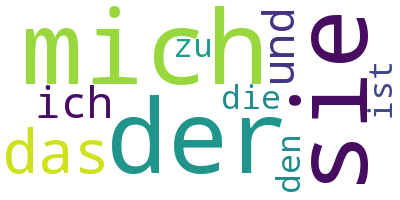
\includegraphics[width=240px]{/Users/Florian 1/Applications/Source_Tree/web-rcat/flask_app/data_user/36bf6974-1bdd-11e8-af65-600308993272_temp_folder/wordcloud_for_single_character1.png}%
\caption{word cloud of "Settembrini"}%
\end{figure}

%


\begin{figure}[H]%
\centering%
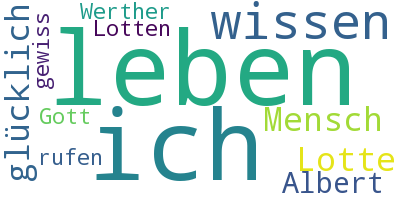
\includegraphics[width=240px]{/Users/Florian 1/Applications/Source_Tree/web-rcat/flask_app/data_user/36bf6974-1bdd-11e8-af65-600308993272_temp_folder/wordcloud_for_single_character2.png}%
\caption{word cloud of "Naphta"}%
\end{figure}

%
\section{Word Cloud for character pairs (method: most frequent contexts words}%
These word clouds were constructed based on most frequent words. They show the most frequent words that appear in the context of the character pair. %


\begin{figure}[H]%
\centering%
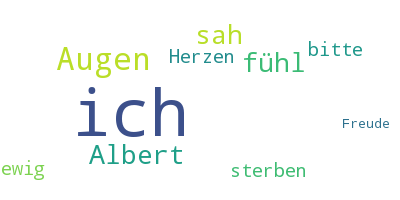
\includegraphics[width=240px]{/Users/Florian 1/Applications/Source_Tree/web-rcat/flask_app/data_user/36bf6974-1bdd-11e8-af65-600308993272_temp_folder/wordcloud0.png}%
\caption{word cloud of "Hans Castorp {-}{-} Settembrini"}%
\end{figure}

%


\begin{figure}[H]%
\centering%
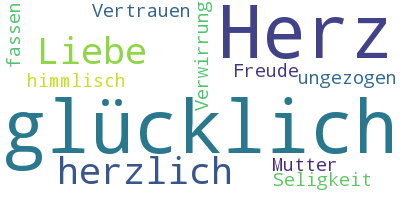
\includegraphics[width=240px]{/Users/Florian 1/Applications/Source_Tree/web-rcat/flask_app/data_user/36bf6974-1bdd-11e8-af65-600308993272_temp_folder/wordcloud2.png}%
\caption{word cloud of "Hans Castorp {-}{-} Madame Chauchat"}%
\end{figure}

%


\begin{figure}[H]%
\centering%
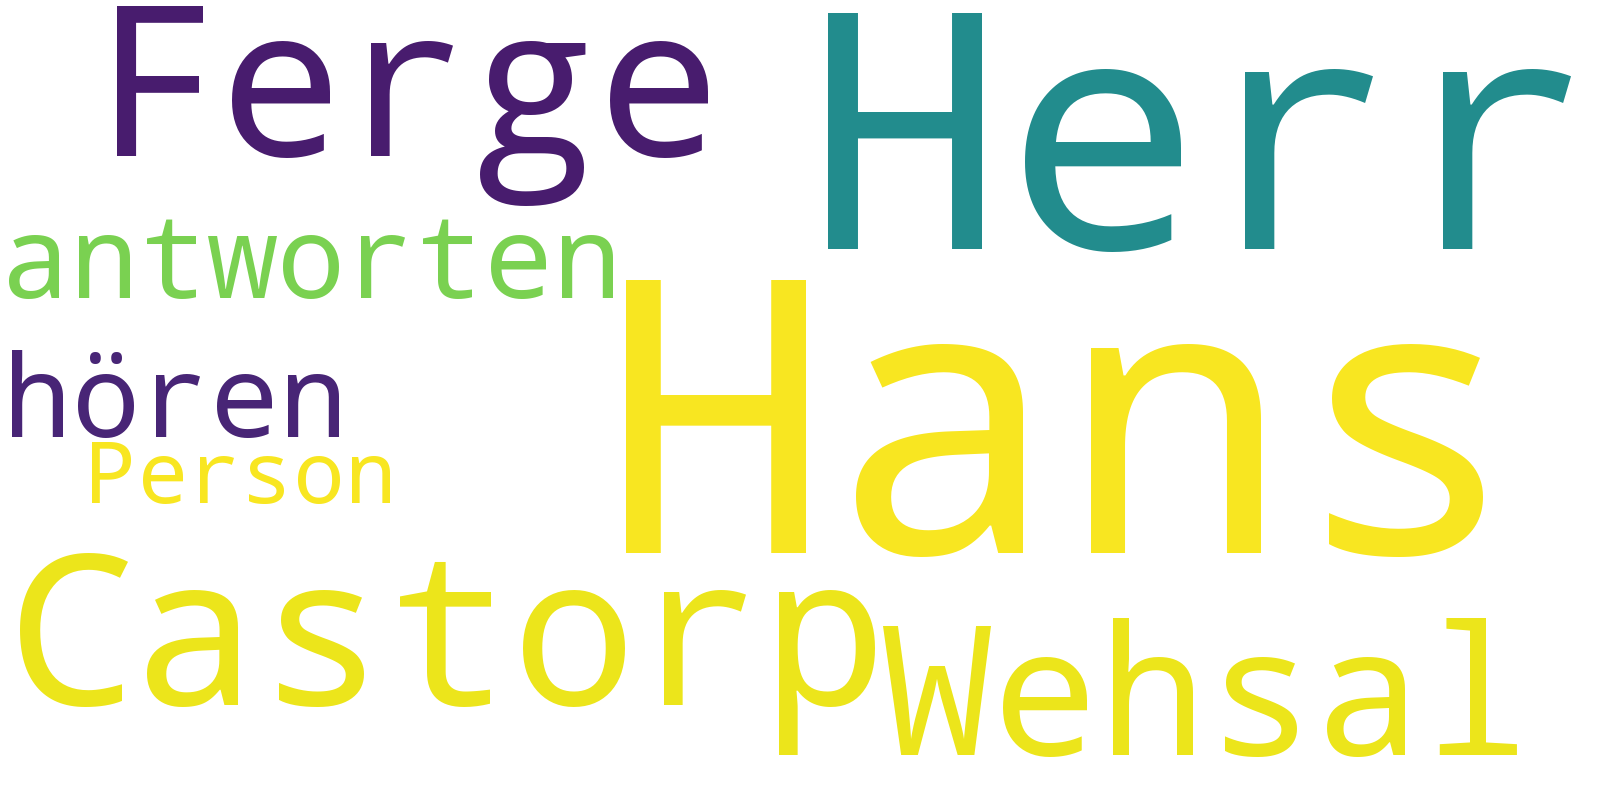
\includegraphics[width=240px]{/Users/Florian 1/Applications/Source_Tree/web-rcat/flask_app/data_user/36bf6974-1bdd-11e8-af65-600308993272_temp_folder/wordcloud17.png}%
\caption{word cloud of "Settembrini {-}{-} Naphta"}%
\end{figure}

%
\section*{rCat, v.0.1}%
This program is developed by Florian Barth and Evgeny Kim with the help of Roman Klinger and Sandra Murr. It is part of the Center for Reflected Text Analytics (CRETA) at the Universtiy of Stuttgart.\newline%
\newline%
Feel free to contact us:%
\begin{itemize}%
\item%
rcat@ims.uni{-}stuttgart.de%
\end{itemize}

%
\end{document}